\documentclass{article}
\usepackage[T1]{fontenc}
\usepackage{times}
\usepackage{geometry}
\geometry{a4paper,left=0.6cm,right=0.7cm,top=1.5cm,bottom=1cm,columnsep=0.8cm}
\usepackage[utf8]{inputenc}
\usepackage{textcomp}
\usepackage{newtxtext}
\usepackage{fontawesome}          % icônes de base seulement
\usepackage[hidelinks]{hyperref}
\usepackage{multicol}
\usepackage{tikz}
\usepackage{hyphsubst}
\usepackage{moresize}
\usepackage{hyphenat}
\usepackage{tabularx}
\usepackage{ragged2e}
\usepackage{xcolor}
\usepackage{enumitem}
\usetikzlibrary{calc, positioning}
\newcolumntype{Y}{>{\RaggedRight\arraybackslash}X}

% icônes manquantes -> puce
\makeatletter
\@for\sym:=faBrain,faMicrochip,faHandshakeO,faTools,faNetworkWired,%
             faDatabase,faServer,faGit,faUsers,faComments,faCalendar,faGroup\do{%
  \@ifundefined{\sym}{\expandafter\newcommand\csname\sym\endcsname{\textbullet}}{}}
\makeatother

% couleurs
\definecolor{maincolor}{HTML}{f0fafc}
\definecolor{seccolor}{HTML}{ffffff}
\definecolor{gray}{HTML}{8c94a9}
\definecolor{sidetext}{HTML}{59cee5}

% bande latérale bleue
\usepackage{eso-pic}
\AddToShipoutPictureBG{%
  \begin{tikzpicture}[remember picture,overlay]
    \fill[maincolor] (current page.north west) rectangle
                     ([xshift=0.3\paperwidth] current page.south west);
  \end{tikzpicture}%
}

% listes
\setlist[itemize]{itemsep=-2pt,topsep=0pt,leftmargin=1.08cm}
\renewcommand{\labelitemi}{\textcolor{sidetext}{\footnotesize$\bullet$}}

\setlength{\parindent}{0pt}
\usepackage{paracol}
\columnratio{0.3}

\begin{document}
\pagestyle{empty}

\begin{paracol}{2}
% ────────────────────────────────────────
% Colonne gauche
% ────────────────────────────────────────
\color{sidetext}
\vspace*{-0.5cm}


\noindent
\begin{minipage}{\linewidth}
  \centering
  \ifx\relax5622990426624a15874c5f69fcd8ff90.jpg\relax\else
  \begin{tikzpicture}
    \clip (0,0) circle (1.5cm) node[anchor=center]
      {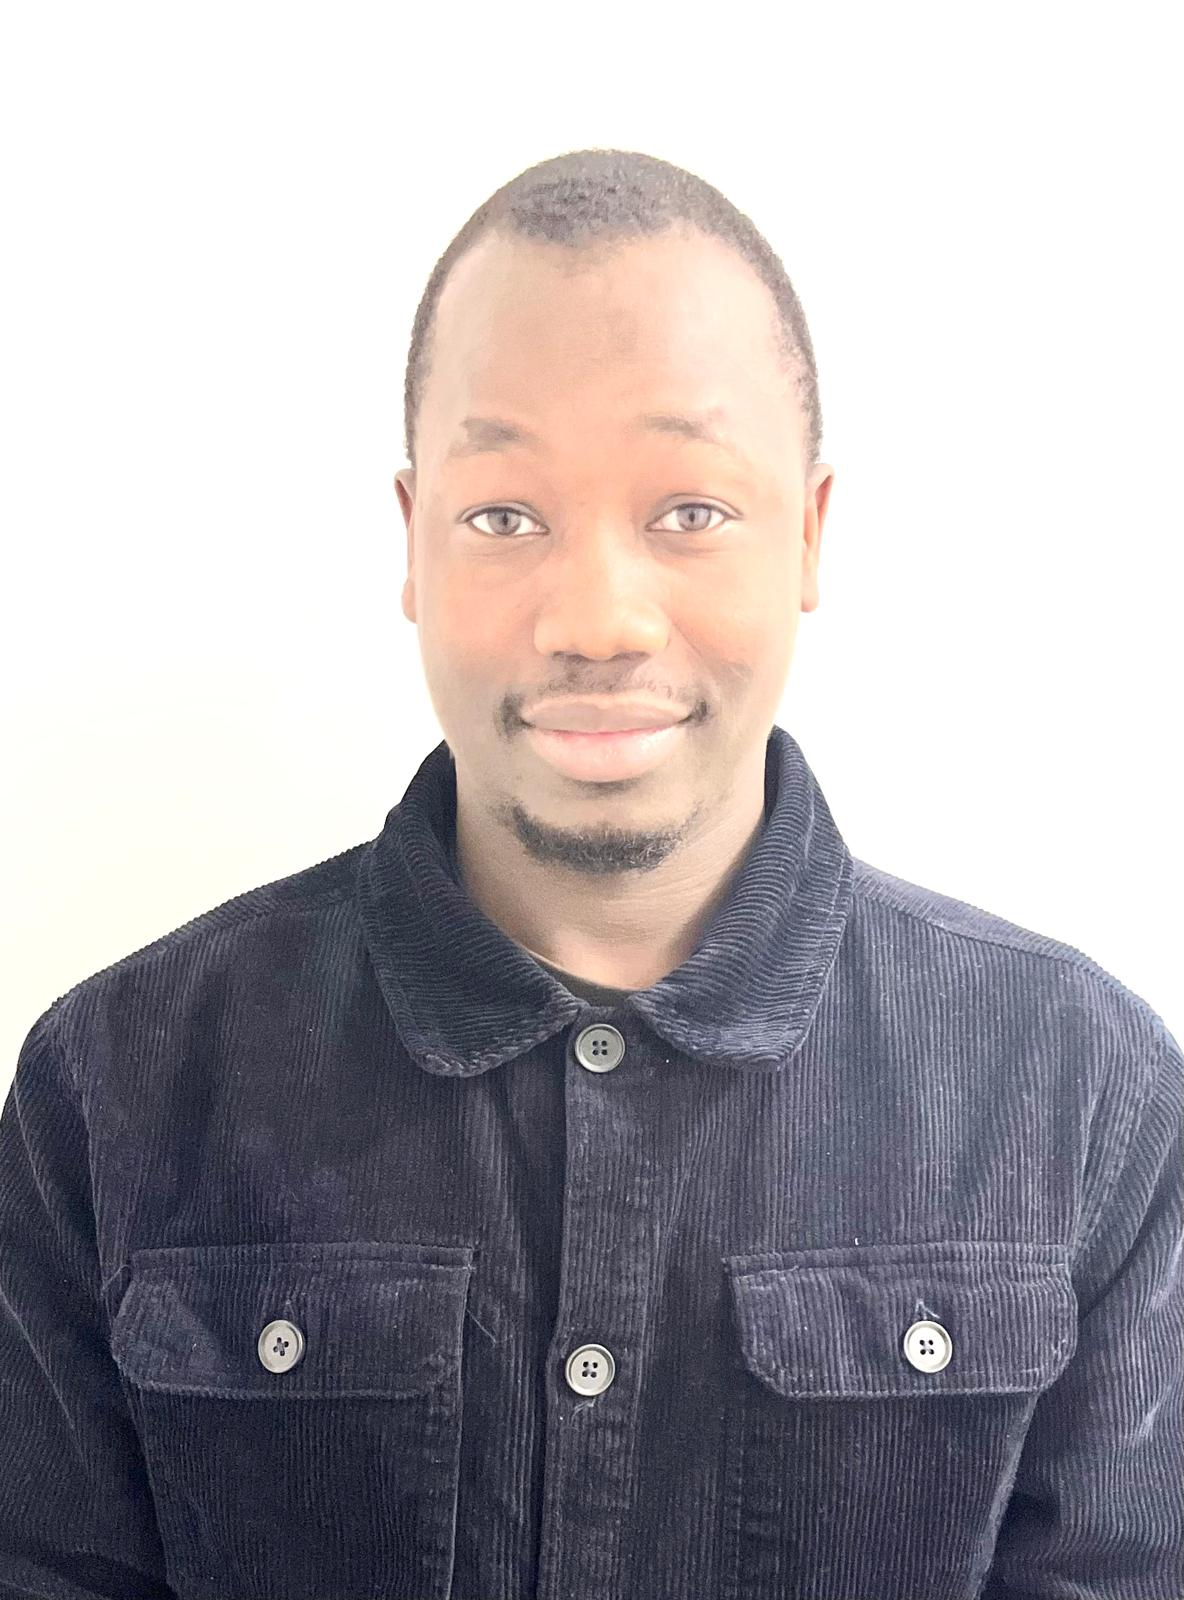
\includegraphics[width=3cm]{5622990426624a15874c5f69fcd8ff90.jpg}};
  \end{tikzpicture}
  \fi

  \vspace{3mm}
  {\color{black}\LARGE \textbf{Judikael Mourouvin}}

  \vspace{1mm}
  {\large Technicien informatique \& marketing digital}

  \vspace{3mm}
  {\color{gray}\rule{\linewidth}{0.4pt}} \\
\end{minipage}

% ── Coordonnées
\begin{tabular}{@{}c l}
  \faPhone &
  \begin{tabular}[t]{@{}l@{}}
    {\color{gray}Téléphone} \\ +590690911448
  \end{tabular} \\
  \\
  \faLinkedin &
  \begin{tabular}[t]{@{}l@{}}
    {\color{gray}LinkedIn} \\
    \href{}{}
  \end{tabular} \\
  \\
  \faMapMarker &
  \begin{tabular}[t]{@{}l@{}}
    {\color{gray}Adresse} \\ Route de Cocoyer \\ 97190 Gosier
  \end{tabular} \\
  \\
  \faEnvelope &
  \begin{tabular}[t]{@{}l@{}}
    {\color{gray}Email} \\
    \href{mailto:jkmou971@gmail.com}{jkmou971@gmail.com}
  \end{tabular} \\
\end{tabular}

\vspace{2mm}
{\color{gray}\rule{\linewidth}{0.4pt}} \\

% ── Langues --------------------------------------------------------
{\color{black}{Langues}}

\vspace{2mm}
\begin{itemize}[leftmargin=*]
\item English - \textcolor{gray}{}
\item Espagnol - \textcolor{gray}{}\end{itemize}          % ← le placeholder va contenir \begin{itemize}…\end{itemize}
\vspace{2mm}
{\color{gray}\rule{\linewidth}{0.4pt}} \\

% ── Compétences ----------------------------------------------------
\vspace{2mm}
{\color{black}{Compétences Clés}}

\vspace{2mm}
\begin{itemize}[leftmargin=*]
\item Administration
\item Réseaux
\item Support
\item Maintenance
\item Marketing
\item Digital
\item Assistance\end{itemize}              % ← idem, une vraie liste
\vspace{2mm}
{\color{gray}\rule{\linewidth}{0.4pt}} \\

% ── Centres d'intérêt
\vspace{2mm}
{\color{black}{Centres d’intérêt}}

\vspace{2mm}
\begin{itemize}[leftmargin=*]
\item Lecture
\item Sport
\item Musique
\item Voyage
\end{itemize}     % ← simple itemize ou tabular

\vfill
~

% ────────────────────────────────────────
\switchcolumn
% Colonne droite
% ────────────────────────────────────────
\color{black}

% ── Profil
\textcolor{black}{\Large \textbf{Profil Professionnel}} \\[2pt]
Passionné par l’informatique et le marketing digital, j’allie compétences techniques et sens de la communication. Mon alternance à la DSI de la Mairie du Gosier m’a permis de conduire des projets numériques, de former les utilisateurs et de renforcer la stratégie digitale. Rigoureux et orienté résultat, je souhaite désormais mettre cette double expertise au service de nouveaux défis à temps plein. \\[8pt]

% ── Expérience
\textcolor{black}{\Large \textbf{Expérience Professionnelle}} \\[2pt]
\colorbox{maincolor}{%
  \begin{minipage}{\linewidth}
    \noindent
    \textbf{Alternant en marketing digital}\hfill 09/2023 - 08/2024\\
    Mairie du Gosier – DSI\\[-0.3em]
    \begin{itemize}[leftmargin=*]
      \item Géré des projets numériques pour optimiser les services municipaux \item Déployé des solutions adaptées après analyse des besoins utilisateurs \item Assuré le support et la formation des agents et contribué à la stratégie digitale
    \end{itemize}
  \end{minipage}}

\vspace{3mm}

\colorbox{maincolor}{%
  \begin{minipage}{\linewidth}
    \noindent
    \textbf{Animateur de la zone informatique}\hfill 06/2022 - 08/2023\\
    Pôle emploi, Gosier\\[-0.3em]
    \begin{itemize}[leftmargin=*]
      \item Assuré le support technique quotidien des conseillers et demandeurs \item Configuré et maintenu le parc informatique pour garantir la disponibilité \item Diagnostiqué et résolu les incidents afin de réduire les interruptions de service
    \end{itemize}
  \end{minipage}}

\vspace{3mm}

\colorbox{maincolor}{%
  \begin{minipage}{\linewidth}
    \noindent
    \textbf{Stagiaire informaticien}\hfill 03/2020 - 08/2021\\
    Numerika, Baie-Mahault\\[-0.3em]
    \begin{itemize}[leftmargin=*]
      \item Configuré, entretenu et sécurisé les équipements informatiques \item Assisté les utilisateurs sur site et à distance
    \end{itemize}
  \end{minipage}}   % ← blocs \colorbox{maincolor}{\begin{minipage}…}

\vspace{8mm}

% ── Formation
\textcolor{black}{\Large \textbf{Formation}} \\[2pt]
\colorbox{maincolor}{%
  \begin{minipage}{\linewidth}
    \noindent
    \textbf{Bachelor Marketing Digital}\hfill 09/2023 - 08/2024\\
    CFA IUTS\\[-0.3em]
    \begin{itemize}[leftmargin=*]
      \item Stratégies de communication digitale, SEO/SEA, analyse de trafic et réseaux sociaux
    \end{itemize}
  \end{minipage}}

\vspace{3mm}

\colorbox{maincolor}{%
  \begin{minipage}{\linewidth}
    \noindent
    \textbf{BTS Systèmes Numériques option Informatique et Réseaux}\hfill 09/2019 - 06/2021\\
    Lycée de Chevalier Saint-Georges, Abymes\\[-0.3em]
    \begin{itemize}[leftmargin=*]
      \item Architectures réseau, systèmes d’exploitation, maintenance matérielle et développement embarqué
    \end{itemize}
  \end{minipage}}       % ← lignes tabular par diplôme

\end{paracol}
\end{document}

